\chapter{Motivation}

%	bpmn introduce
	Business processes are fundamental elements for companies and organizations. They aggregate all the tasks, activities, and timelines involved in companies' workflow whose aim is to provide business services or to create value \cite{literature_review_2}. Business Process Modeling Notation, also known as BPMN is a modeling language describing such workflows by using graphical notations and thus provides an easily understandable overview of the operations performed in the organization for all business users \cite{literature_review_1}. 
	
	Due to the importance of Business processes, leveraging the BPMN techniques can positively affect an organization's performance. Organizations can flexibly adapt to constantly changing business conditions through business process management by providing processes standardization, improvement and quick execution of the activities. \cite{t2m_5} However, not everyone is familiar with the BPMN designing techniques. Consequently, managers, along with other process participants prefer using natural language to define business processes. As a result, organizations usually have a large amount of information stored as text documents \cite{literature_review_2}. However, process modeling is not a simple task, but it is time-consuming, and experts with professional knowledge are required. According to \cite{t2m_5}, process modeling requires 60\% of the time within a business process management project. Adopting the approach that identifies and extracts process models can minimize the time and effort of the process modeling. \cite{literature_review_3} also suggests that  BPMN leads to process improvements, resulting in process cost reduction, quality increment, and higher revenue production. 
	%todo: if there is a need to expand the details of difficulties of process modeling, then refer to literature_review_2 
	
%	nlp introduce
	Over the past years, the development of AI techniques brought solutions to many technical difficulties. Natural Language Processing (NLP), as one of the AI's branches, could possibly address the problem of the difficulties in process modeling. Natural Language Processing is an interdisciplinary discipline focusing on the study of algorithms that enable the computer to understand and process the human language\cite{t2m_3}. During the understanding and processing of the natural language text, NLP performs three types of analysis: Firstly, morphological analysis is performed, which analyze the structure of words. The syntactic analysis then explores the grammar relationship between words in sentences, deciding which grammar category the word belongs to. Finally, semantic analysis is executed, which leverages the afore analyses to define the meaning of the text based on the knowledge of sentence structure and the relationship between words \cite{literature_review_2}. 
%todo: if there is a need to expand the details of NLP analysis, then refer to literature_review_2 introduction part
	
%	why should nlp be used to generate the bpmn
	The unique features of the NLP technique make it very suitable for exploiting information from the text documents that record the firm's business process and then analyzing the data to generate the process models automatically. This paper serves as a proposal to suggest using NLP to extract the information from text written in nature language and automatically generate the corresponding business model.
	
	\section{Research Questions}

	The main research question (\textbf{RQ}) is formulated as: "\textit{How can business process models be automatically generated from textual descriptions using Natural language processing techniques?}". To better answer the main research question, three embedded aspects can be revealed: \textbf{RQ1}: "\textit{Which NLP methods can be used to extract information?}"; \textbf{RQ2}: "\textit{How can the extracted information be analyzed and composed to generate business process models?}" and finally \textbf{RQ3}: "\textit{How does the proposed approach perform with different kinds of input documents?}"

	
	Currently, there exist various tools, libraries, and dependencies for NLP. Therefore, the first research question \textbf{RQ1} tries to figure out which methods are the most suitable ones to use to extract information from textual descriptions. Currently, there exist several Natural language processing tools in academia and industry, and this work wants to explore their strengths and limitations. The work also aims to use the most suitable state-of-art-technique to perform the information extraction from the natural language text documents. 
	In the next step, \textbf{RQ2} explores how can the information in the text descriptions be analyzed and extracted and then be built into the business process model. The activities recognition here is an essential but challenging task here because the identified business activities and actors serve as a basis for the BPMN generation. To address this problem, the work aims to discover the typical structure of the business activities' textual representations in natural language documents by exploring the syntactical and grammatical relationships of the words. Furthermore, reconstructing the extracted business information is also challenging. The work will focus on identifying the conditional and sequential relationships of the business activities to develop algorithms that can generate a business process model with high accuracy.
	The last research question \textbf{RQ3} tries to compare different complexity levels of the natural language documents. This research question aims to discover the adaptability of the proposed approach. The work will reveal the performance of our approach given natural language documents with different complexity levels, e.g., usual textual process descriptions, company policies, legal regulatory documents, and so on. Since such regulatory documents with higher complexity levels are always formulated in a more complex manner. The work should determine whether the explored extraction strategies still apply to such documents and whether the recognition accuracy drops. 
	
\begin{figure}[h]
    \centering
    \caption{Overview of the approach design}
    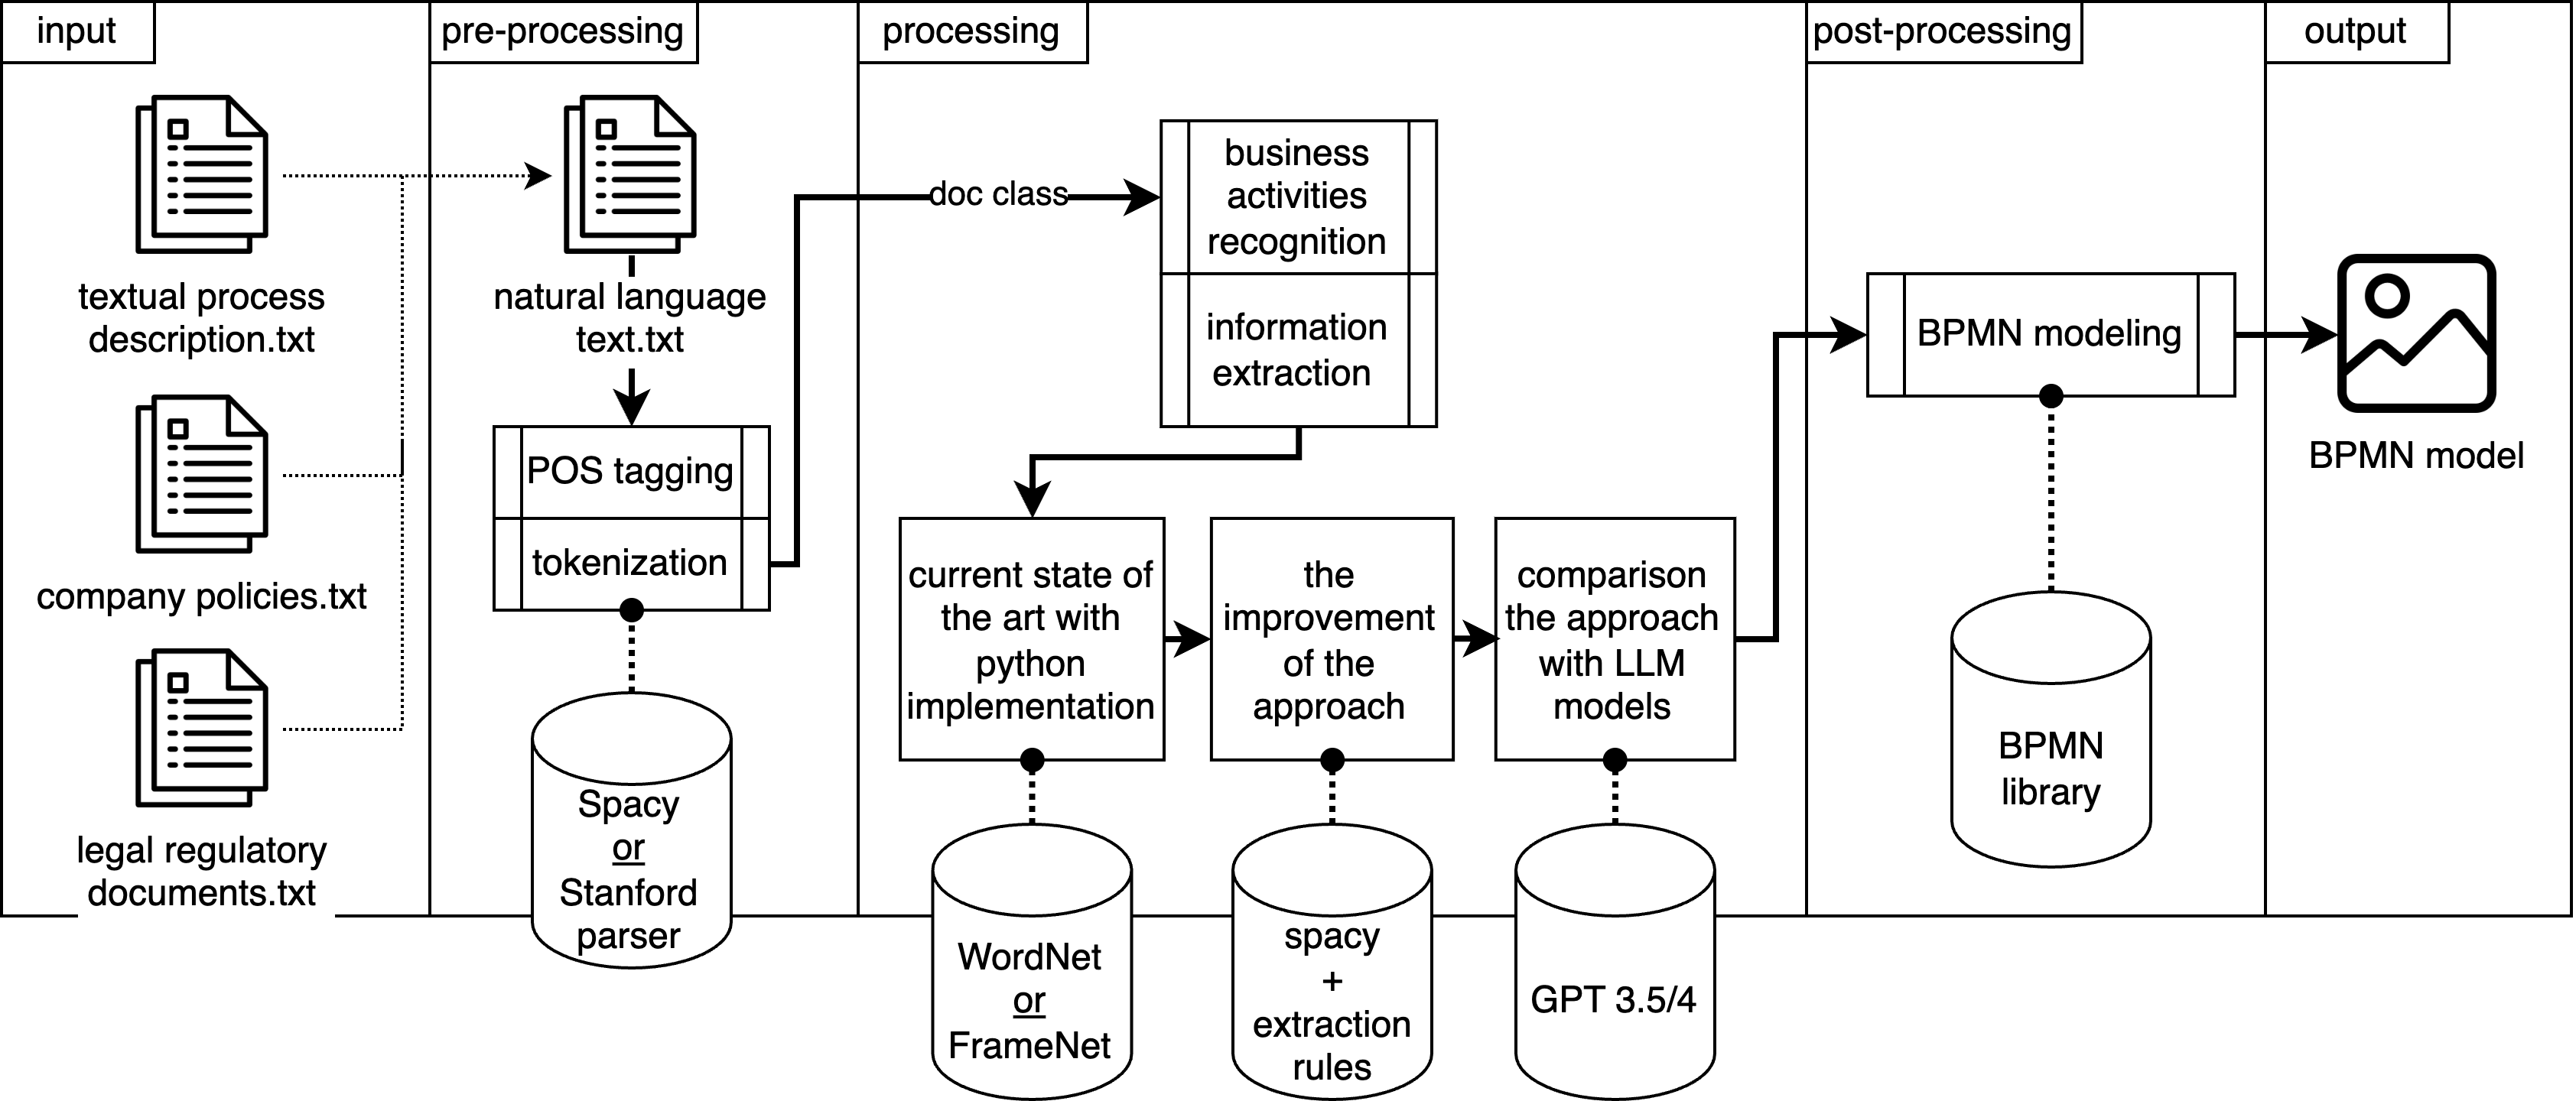
\includegraphics[width=1\textwidth]{tum-resources/images/overview.png}
\end{figure}
	
	